\documentclass[12p]{article}
\usepackage{graphicx}
\usepackage{fancyhdr}
\usepackage{titlesec}
\usepackage{natbib}
\usepackage{outlines}
\usepackage[
  top=1.5cm,
  bottom=1.5cm,
  left=3cm,
  right=3cm,
  headheight=17pt, % as per the warning by fancyhdr
  includehead,includefoot,
  heightrounded, % to avoid spurious underfull messages
]{geometry}
\pagestyle{fancy}
\fancyhf{}
\cfoot{\emph{Mendenhall 18-10: Page \thepage}}
\lhead{\emph{Mendenhall Opportunity 18-10 Proposal}}
\rhead{\emph{William Savran, Ph.D.}}
\titleformat*{\section}{\large\bfseries}
\titleformat*{\subsection}{\bfseries}
\begin{document}

\begin{center}\Large\textbf{Leveraging Machine Learning for Next-Generation Global Earthquake Monitoring}\end{center}

\section*{Overview}
For earthquakes occurring globally, the United States Geological Survey (USGS) National Earthquake Information Center (NEIC) provides a continuous service to determine earthquake source properties, and to share this information with national and international agencies, researchers, and the public. Before source characteristics can be computed and delivered, earthquakes must be detected on the seismic network and their hypocenters determined as accurately and quickly as possible. The NEIC utilizes a data processing pipeline that transforms raw seismic data, recorded globally, into both fully automated and semi-automated data products, such as, earthquake hypocenters, magnitudes, moment tensors, fault slip models, and potential loss and damage information (e.g., \citet{Thompson2019, Michael2019}).

At the core of this process, an association algorithm determines the most probable hypocenter location of a seismic event using arrival time picks from individual stations and an assumed velocity model. The performance of an association depends largely on the ability to detect and characterize seismic signals from individual stations. Recent  studies show deep learning algorithms being used effectively for earthquake detection and for classifying seismic signals using individual station records. Understanding these algorithms in the context of routine processing at the NEIC could significantly improve the detection threshold of the global catalog, and would help to reduce false associations. As such, I propose to build a framework using machine learning to:

\begin{enumerate}\bfseries
  \item Implement algorithms to detect earthquakes and classify source characteristics, toward a better global catalog and
  \item Quantify the improvements from machine-learning algorithms on earthquake detection and association, as compared with previous methods, and
  \item Introduce machine-learning to the routine processing of global and regional seismic data at the NEIC.
\end{enumerate}

The proposal deals primarily with implementing and understanding limitations of deep-learning algorithms as applied to association and earthquake detection, with the goal of improving the global catalog by decreasing the magnitude threshold and improving completeness. Due to a dearth of recordings from significant domestic earthquakes, research and operational knowledge gained from studying earthquakes globally can be applied domestically. Thus, improving our ability to detect and characterize earthquakes globally can influence domestic activities such as operational earthquake forecasting, earthquake early warning, and future versions of the National Seismic Hazard Map. The proposed work will contribute to our understanding of global and domestic earthquakes and advance the earthquake monitoring capabilities at the NEIC.

This proposal is motivated by the NEIC Strategic Plan, (2019-23, Circular 1457; \cite{Hayes2019sp}) specifically to ``finalize improvements to its regional monitoring capabilities, including the implementation of a variety of improved earthquake detection and association algorithms" and ``to explore the benefits of machine learning for improved earthquake detection and source characterization." The work will be conducted at USGS NEIC in the Golden, Colorado office under the direct supervision of William Yeck with advisors Paul Earle, David Shelly, Gavin Hayes, Michelle Guy, Harley Benz, and Zachary Ross.

\section*{Background Information}
\subsection*{Earthquake Monitoring: Detection and Association}

The NEIC receives continuous seismic data from over 2000 stations globally (Fig. \ref{fig:stations}). Earthquake monitoring involves using seismic signals observed at multiple stations to determine hypocenters and produce producing containing information about an earthquake source. This process must occur autonomously and produce results that are reliable and timely per the USGS's responsibility to ``provide timely information to other agencies, emergency managers, the media, and the public about hazardous events as they occur" \citep{Holmes2013}.

The NEIC uses Hydra \citep{Patton2016} to manage the processing pipeline from earthquake detection through source characterization and analyst intervention using graphical user interfaces. Hydra uses a detection algorithm known as the Hydra Picker which implements the classic short-term average (STA) / long-term average (LTA) \citep{Lee1981} technique to detect picks in continuous seismic data. The major drawbacks of STA/LTA are the inability to distinguish between source types including phases and other characteristics of the source, and the sensitivity of the outputs to the tuning parameters. In other words, picks from STA/LTA algorithms have ambiguous phase and provide no constraints on possible source location aside from arrival times. Improvements in detection algorithms will significantly improve our ability to detect smaller earthquakes, and will help to improve catalog completeness.

Phase ambiguous picks made by the Hydra Picker can be processed by the Global Associator 3 (GLASS3; \citet{Yeck2019}) algorithm, which provides a solution to the association problem across global, regional, and local scale networks. GLASS3 accomplishes this by defining so called association webs which consist of association-nodes (potential source locations), sites (seismic stations), and configurable parameters necessary to define nucleation criteria. Association-nodes are regularly spaced, defined by their latitude, longitude and depths, and represent an exhaustive set of possible source locations. The nodes link to the closest sites via travel times computed using an assumed velocity model. Once the network has detected a pick, it iteratively tries to either associate the pick with a previous hypocenter or nucleate the pick to generate a new trial hypocenter. Since association nodes are regularly spaced, both nucleation and association can be improved by including additional information with a pick to help constrain the possible source location in space. By knowing a priori the depth, back azimuth and source-distance, we can limit the nodes where picks can associate and nucleate. Thus, providing additional constraints to the association algorithm is an obvious step to reducing failed associations and improving earthquake detection capabilities.

\begin{figure}[!htb]
  \center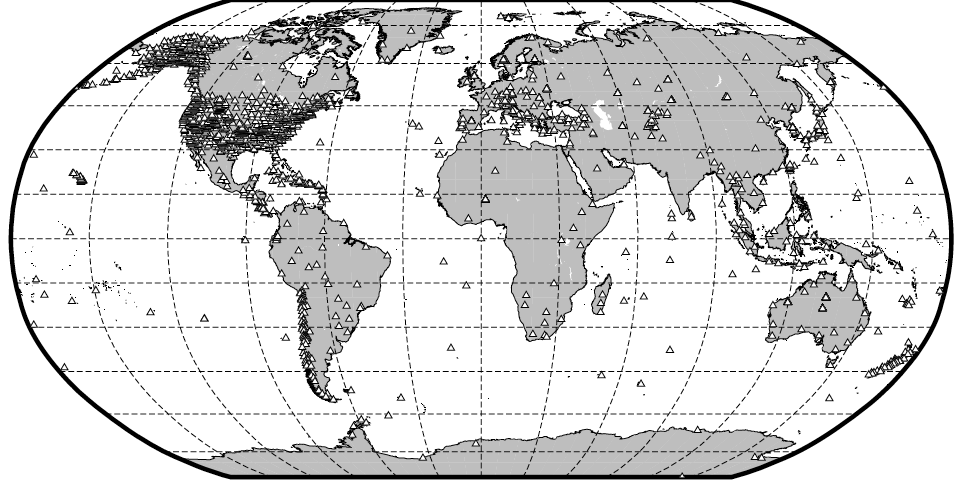
\includegraphics[width=0.8\textwidth]{figures/global_station_coverage.png}
  \caption{\label{fig:stations} From \cite{Yeck2019}: As of 25 June 2018, 2032 unique seismic stations provide real-time data to the NEIC (shown using white triangles).}
\end{figure}

\subsection*{Deep Neural Networks for Earthquake Detection and Source Characterization}

Within the last few years advancements in the field of machine-learning have drastically improved our ability to make inferences from data, especially for tasks that previously required a human brain \citep{Lecun2015}. In general, machine-learning algorithms approximate a function that provides a mapping from input to output values. Fully connected neural-networks (FCNNs) consist of fully connected layers of neurons whose architecture depends on the the problem being solved and the dimensionality of the input and output values. The first layer of an FCNN accepts `features' of the data and the final layer contains the desired outputs or labels. Using ground-motion prediction equations as an example, features are source-receiver distances and magnitudes while outputs are peak ground metrics or spectral accelerations. Furthermore, there can be an arbitrary number of `hidden' layers between the input and output layers. The performance of FCNNs depends on the choices of the features extracted from the data, which are typically engineered manually and can be difficult to constrain. NNs with large numbers of layers (and therefore parameters) are referred to as deep networks.

Convolutional neural networks (CNNs) have the ability to automatically learn features by performing a series of convolution and pooling (downsampling) operations to distill raw input data into a concise feature vector (Fig. \ref{fig:cnn}). The extracted feature vector then feeds into a standard FCNN to perform inference tasks. The filter parameters of the convolutional layers are learned during the training process, meaning that CNNs act as fully-automated feature engineering systems. The CNN approach requires vast amounts of data to properly train the models and avoid overfitting, because deep network architecture can have millions of free parameters. Due to their ability to extract features from raw data, CNNs have been used successfully in seismology to, for example, (1) detect and locate earthquakes in the central United States \citep{Perol2018}, (2) determine P-wave arrival times and first-motion polarity \citep{Ross2018a}, (3) perform generalized phase detection of P- and S-waves \citep{Ross2018b, Zhu2019a}, and (4) de-noise seismic recordings \cite{Zhu2019b}, amongst other applications. CNNs can be used to make other inferences assuming sufficient training data exists with the appropriate labels.

\begin{figure}[!htb]
  \center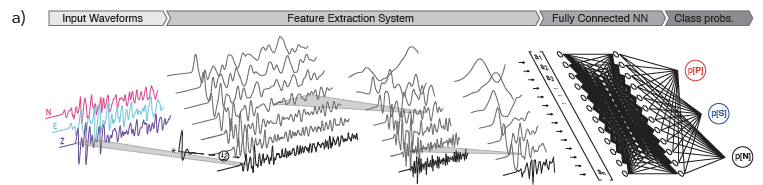
\includegraphics[width=\textwidth]{figures/cnn_architecture_ross2018a.png}
  \caption{\label{fig:cnn} From \cite{Ross2018b}: Cartoon depicting CNN used for generalized phase detection. The illustration shows input waveforms undergoing a series of convolution and downsampling operations to extract usable features and the coupling of the CNN and the FCNN.}
\end{figure}

In seismology, we have the fortune of high-quality labeled datasets continuously updated an expanded through the expert review of NEIC analysts. The canonical form of this data can be accessed through the USGS Preliminary Determination of Epicenters (PDE) bulletin, which contains the human-reviewed events, their associated picks and metadata. Each pick of an event in the PDE contains phase information, station-event distances, station-event azimuths, and event depths. Therefore it is straightforward to extend the CNN architecture proposed by \citet{Ross2018b} for Generalized Phase Detection (GPD) to classify properties of picks that can be used to help constrain the association problem and make inferences on the .

\section*{Using Machine Learning for Earthquake Detection and Association}

The work proposed here is two-fold: (1) to implement and deploy machine-learning based detectors (e.g., \citet{Perol2018} or \citet{Ross2018a}) to supplement currently used methods such as STA/LTA pickers and (2) to implement machine-learning algorithms to classify event-station azimuths, event-station distances, and event depths to help constrain associations made by GLASS3. As the work proposed here is intended to be operationalized, a significant component of the work will involve making rigorous comparisons between these machine-learning algorithms and the currently used approaches. Items (1) and (2) relate naturally resulting in a classification framework that utilizes machine-learning for the detection and association of phase picks with the ultimate goal of lowering magnitude thresholds and improving completeness globally.

The first step is therefore to obtain continuous waveform data associated with each of the events and picks in the PDE bulletin and associated labels used for classification. Based on automated picks from the STA/LTA picker we will store 60 seconds of continuous waveform data centered on the pick time. We will preprocess the three-channel raw seismic data set following \citep{Ross2018b} which involves de-trending the data within the window and high-pass filtering above 1 Hz to remove microseismic signals. The data will be resampled to 100 Hz, and if necessary, acceleration records will be integrated to velocity. Further processing will be necessary depending on the classification task, specifically, adjusting the window length of the raw data. Additionally, 3-channel data amplitudes should be normalized by the maximum amplitude within the window from any channel. Azimuths and depths will be transformed to categorical variables so the inference can be posed as a classification problem. Augmentations within data windows will be performed, such as reversing polarizations and swapping horizontal components and uniformly shifting the pick time within the window. This results in a larger data set to help the model generalize.

The next step is implementing CNNs used to provide constraints to the association problem, as this will likely be a necessary prerequisite to deal with the increased pick volume resulting from a CNN picker (e.g., \citep{Perol2018}). Furthermore, a GPD algorithm can be applied directly as a detector, because the model is trained to distinguish between P-waves, S-waves and noise. The azimuth, depth, and distance classifiers will map raw waveform data associated with STA/LTA picks into finite depth, azimuth, or distance bins. The classification accuracy might not match the performance of phase-classification as the features associated with these new labels are presumably more ambiguous across the data set. As a test to increase model performance, we could follow the approach of \citet{Zhu2019b} to compute spectrograms to use as input data to the CNN. Including frequency information, in addition to temporal information, provides more data for the CNN feature extraction system to leverage. However, the additional computational cost of computing spectrograms will need to be weighed against its usefulness.

For the classification tasks proposed here, we will implement the architecture and training procedure following \citet{Ross2018b}. The network will consist of four convolutional layers and two fully connected layers using rectified linear units as activation functions. Batch normalization will be applied to each layer. An important step in training the CNNs will be determining the appropriate hyper-parameters to use for the model and the data augmentation required to produce a reliable testing/training set. Hyper-parameter adjustments are typically made using a trial-and-error approach and confirming results based on cross-validation of testing data. Data will be divided into testing and training sets using 75\% and 25\% of the data respectively. The model will be trained using a cross-entropy loss function with the ADAM optimization algorithm. The training will be terminated when the validation loss has not decreased in more than five training epochs.

Model performance will be assessed using the standard approaches for evaluating classification algorithms. Since CNNs output classification probabilities some arbitrary threshold must be set to indicate a classification. As such, the probability values associated with the classification threshold will need to be calibrated appropriately. We can assess the model performance by comparing precision and recall curves for different probability thresholds. Admittedly, most choices of classification thresholds are largely arbitrary. Additionally the F$_1$ score (harmonic mean of precision and recall) can be used as a synoptic view of model performance at a given probability threshold.

Once the CNNs have been trained and shown to produce classifications with sufficient precision and recall, their outputs will be fed into GLASS3 to assess their impact on the association problem. Each pick provided to GLASS3 will now contain the azimuth, depth, distance, and phase in addition to the arrival time. The picks and their new metadata will be used to limit the GLASS3 association-nodes where rupture is allowed to nucleate. The GLASS3 algorithm may need to be extended by allowing for a dynamic list of supported association-nodes for a given site conditional on the pick metadata. Therefore, when attempting nucleation of a pick the algorithm can use a subset of the previously supported nodes for triggering nucleation, increasing computational efficiency and reducing false associations. Additionally, similar techniques could be applied when attempting to associate picks with previous hypocenters. The outputs from GLASS3 using classification constraints must be compared against the unconstrained case with the goal of quantifying the improvements of the association problem. I propose to follow a similar approach as \citet{Yeck2019} to compare GLASS3 with constrained GLASS3. Initial metrics for comparison will be the spatial locations of the detected events from constrained and unconstrained GLASS3 solutions and the relative percents of PDE events detected as a function of the pick metadata.

Next, I propose to evaluate a CNN trained to detect seismic signals in continuous seismic data. Based on results from \citet{Perol2018} and \citet{Ross2018b} we can expect potentially an order of magnitude more detected events assuming the regional and local results transfer to the global network. There are two possible ways to implement this CNN picker. First, we could follow the GPD approach from \citet{Ross2018b}, which would directly transfer from the work classifying picks. Or a more advanced network architecture using sequence-to-sequence learning that combines convolution layers with long-short-term memory (LSTM) layers \citep{Mousavi2019}. For consistency with our previous work, it's sensible to follow the network architecture implementation and training strategy proposed for the classification framework. While more advanced networks like the CNN+LSTM model might improve detection over a standard CNN approach, those improvements are left for future work.

Phase-picks determined from the CNN picker will be fed into the classification framework developed to improve GLASS3 associations. As before, picks and their associated metadata will be used by the GLASS3 association algorithm to determine probable hypocenter locations. A similar verification will be performed except now we must (1) compare unconstrained GLASS3 with STA/LTA picks with unconstrained GLASS3 with CNN picks, and (2) compare the constrained GLASS3 outputs with STA/LTA picks and constrained GLASS3 outputs with CNN picks following \citet{Yeck2019}. It will be interesting to determine the changes in magnitude of completeness and detection threshold when using CNNs for both picking and constraining association. We anticipate that the best association performance (and global catalog quality) comes from using a CNN picker and constraining GLASS3. Therefore, introducing a CNN picker and classification framework for the association problem has the potential to drastically improve current global monitoring capabilities at the NEIC.

\section*{Summary and Future Impacts}
This proposal contains both research and operational components focused on incorporating machine-learning algorithms to improve global earthquake monitoring at the NEIC. The proposed classification framework complements current work being  at the NEIC and provides a natural extension for improvements to the GLASS3 association algorithm \citep{Yeck2019}. A major goal of this work involves incorporating these algorithms into the routine processing of global seismic data. The foundation of all source products (e.g., moment magnitude, moment tensor, slip model) depends on quick and accurate hypocenter locations, therefore advances made to earthquake detection and association have the potential improve all related source products.

This work focuses on the global network but future work would be to apply these techniques to regional and local association webs to understand the effects on improving monitoring capabilities domestically and during aftershock sequences. A natural evaluation of this work would be to use machine learning algorithms to help develop additional source products such as moment tensors (e.g., \citet{Ross2018a}) and facilitate efforts for earthquake early warning (EEW). Due to their ability to extract features from raw data, it remains conceivable that seismic waveform data could be used to predict quantities useful for EEW, such as PGV, PGA, or magnitudes assuming that ideas of weak determinism hold \citep{Goldberg2018}. While this is outside the scope of work presented here, this would be an interesting avenue for future applications of machine-learning. Thus, the expected outcomes from this proposal have the capacity to drastically improve operational capabilities at the NEIC well into the future.

\section*{Links to USGS Science Program Strategy}
The proposed work is motivated by the USGS Science Strategy \citep{Holmes2013} and the NEIC Strategic Plan \citep{Hayes2019sp} to:

\begin{enumerate}
  \item \emph{``Take advantage of rapidly changing technology, recognizing that the ability to monitor effectively depends on the technology used and the ability to adapt to changes."} - Advancements in machine-learning provide automated tools that have been shown to replicate the performance of humans in complex classification tasks. Applying these toward seismic monitoring will improve our ability to detect earthquakes and strengthen our earthquake response products.

  \item \emph{``Evaluate warning and response products to improve their accuracy, timeliness, and communication, and demonstrate the value of the USGS hazard investment in observations and fundamental understanding."} - Accurate and reliable event detections lie at the heart of all earthquake response products. Thus, improvements made to our ability to detect earthquakes cascade into other response products.

  \item \emph{``Promote targeted research on physical hazard initiation processes, because limited understanding about these processes limits the ability to make accurate predictions."} - Our ability to observe seismicity in the earth is limited by the amount of stations we provide and our ability to process the recorded data. Machine-learning approaches to earthquake monitoring have the capability to encourage new research on process before earthquakes. For example, \citet{Trugman2019} discovered pervasive foreshock activity in southern California using catalogs enhanced by machine-learning.

  \item \emph{``Use machine-learning to improve monitoring operations at the NEIC"} - The proposed work has obvious implications for improving monitoring operations at the NEIC and will provide a framework to allow for additional machine-learning based approaches to be incorporated in the future.

\end{enumerate}

\section*{Required Scientific Facilities}
The proposed work requires access to facilities with GPU accelerated computing to train the deep neural-networks. \citet{Ross2018b} required three NVIDIA GTX1060 graphics cards for their training needs. Both the USGS Yeti Supercomputing cluster and the USGS Tallgrass cluster provide GPU computing that should be sufficient to complete the proposed work.

\bibliographystyle{plainnat}
\bibliography{references}

\end{document}
